\documentclass[t, 10pt, aspectratio=169, table, x11names]{beamer}
\usetheme{metropolis}

\usepackage{xcolor}
\usepackage[utf8]{inputenc}
\usepackage[default]{lato}
\usepackage[T1]{fontenc}
\usepackage{lmodern}
\usepackage{listingsutf8}
\usepackage{hyperref}
\usepackage{wrapfig}
\usepackage{dsfont}
\usepackage[export]{adjustbox}
\usepackage{array, booktabs}
\usepackage{cellspace}

\graphicspath{{./resources}}
\lstset{inputpath=./resources, xleftmargin=7mm, xrightmargin=7mm}

\definecolor{codegreen}{rgb}{0,0.6,0}
\definecolor{codegray}{rgb}{0.5,0.5,0.5}
\definecolor{codepurple}{rgb}{0.58,0,0.82}
\definecolor{backcolour}{rgb}{0.95,0.95,0.92}
\hypersetup{colorlinks,urlcolor=blue}

\newcommand{\redhighlight}[1]{{\color{red}\textbf{\texttt{#1}}}}

\newcommand{\R}{\mathds{R}}
\newcommand{\appallingunderline}[1]{
	\underline{\smash{#1}\vphantom{T}}\vphantom{#1}%
}

\lstdefinestyle{sql}{
	backgroundcolor=\color{backcolour},
	commentstyle=\color{codegreen},
	keywordstyle=\color{magenta},
	numberstyle=\tiny\color{codegray},
	stringstyle=\color{codepurple},
	basicstyle=\ttfamily\scriptsize,
	breakatwhitespace=false,
	breaklines=true,
	captionpos=b,
	keepspaces=true,
	numbers=left,
	numbersep=5pt,
	showspaces=false,
	showstringspaces=false,
	showtabs=false,
	tabsize=2
}

\lstdefinestyle{winprompt}{
	backgroundcolor=\color{backcolour},
	commentstyle=\color{codegreen},
	keywordstyle=\color{magenta},
	numberstyle=\tiny\color{codegray},
	stringstyle=\color{codepurple},
	basicstyle=\ttfamily\footnotesize,
	breakatwhitespace=false,
	breaklines=false,
	breakatwhitespace=false,
	prebreak=false,
	captionpos=b,
	keepspaces=true,
	showspaces=false,
	showstringspaces=false,
	showtabs=false,
	tabsize=1
}

\lstset{style=sql}
\lstset{inputencoding=utf8/latin1}


\begin{document}

	\author{Victor Mayrink}
	\title{Curso de SQL}
	\subtitle{Aula 1: Instalação das ferramentas e configuração do ambiente}

	%Frame: title
	\begin{frame}[plain]
		\maketitle
	\end{frame}

	%Frame: agenda
	\begin{frame}
		\frametitle{Agenda}
		\vspace{1cm}
		\begin{enumerate}
			\large
			\item O que é SQL
			\item Por quê aprender SQL?
			\item Instalação e configuração das ferramentas
		\end{enumerate}
	\end{frame}
	

	\section{Índices}

	%Frame: client-server
	\begin{frame}
		\frametitle{Índices - Introdução e Motivação}
		Imagine um antigo cartório de registro civil...
		\bigskip
		\begin{figure}[h]
			\centering
			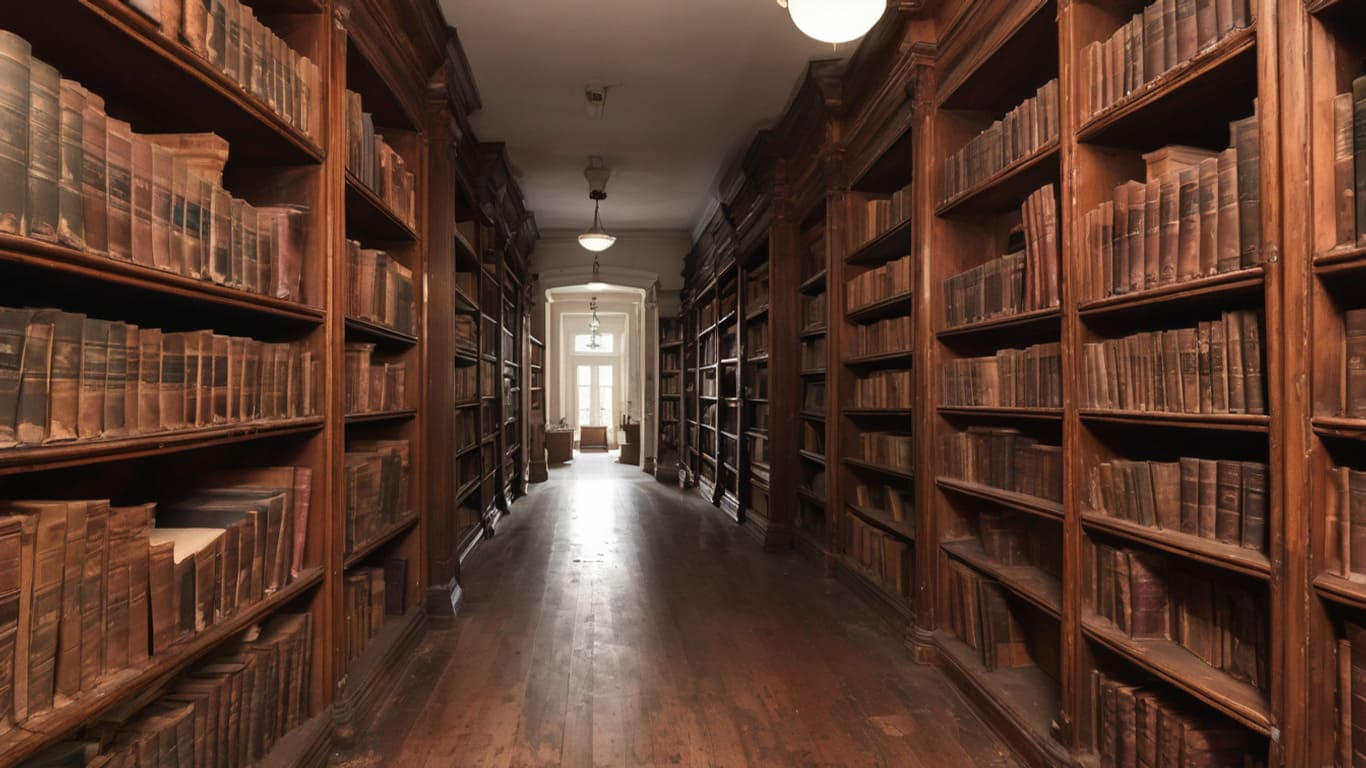
\includegraphics[width=0.65\textwidth]{registry.jpg}
		\end{figure}
	\end{frame}

	%Frame: client-server
	\begin{frame}
		\frametitle{Índices - Introdução e Motivação}
		\begin{itemize}
<<<<<<< Updated upstream
			\item Os  registros de nascimento são armazendos em \textit{livros de registos};
=======
			\item Os registros de nascimento são armazendos em \textit{livros de registos};
>>>>>>> Stashed changes
			\bigskip
			\item Cada registro de nascimento ocupa uma página inteira de um livro. Esses registros contém informações como: nome completo, data de nascimento, local de nascimento, nome da mão, nome do pai, etc.;
			\bigskip
			\item Cada livro possui 500 páginas, enumeradas de 1 a 500;
			\bigskip
<<<<<<< Updated upstream
			\item Os livros são rotulados com um número de sequencial, e depois de completamente preenchidos, ficam guardados em uma prateleira de forma ordenada;
			\bigskip
			\item Ao registrar um novo nascimento, o tabelião sempre utiliza a primeira página em branco disponível;
=======
			\item As lombadas dos livros são rotuladas com um número de sequencial, e depois armazenados em uma prateleira de forma ordenada; (para facilitar adicione na lombada a data do primeiro registro que o livro contém)
>>>>>>> Stashed changes
		\end{itemize}
	\end{frame}

	%Frame: client-server
	\begin{frame}
		\frametitle{Índices - Introdução e Motivação}
		\reasonboxbegin{Regra básica}{MaterialTeal800}
			Ao registrar um novo nascimento, o tabelião sempre utiliza a primeira página em branco disponível;
		\reasonboxend
		\begin{itemize}
			\item Assim, os registros serão \textbf{naturalmente} ordenados conforme a data e hora de registro
			\bigskip
			\item Dessa maneira é fácil localizar um registro, \textit{desde que} você saiba a data em que esse registro foi feito.
			\bigskip
			\item \textit{Quantos nascimentos foram registrados em 17 de Maio de 1868?}
			\bigskip
			\begin{itemize}
				\small
				\item Resposta: Procure o primeiro registro de nascimento desta data e conte quantos registros foram realizados até encontrar o primeiro registro do dia seguinte (excluindo-o da contagem)
			\end{itemize}
		\end{itemize}
	\end{frame}

	%Frame: client-server
	\begin{frame}
		\frametitle{Índices - Introdução e Motivação}
		Mas e se eu precisar procurar o registro de uma pessoa conhecendo apenas o seu \texttt{nome completo}?
		\bigskip
		\begin{columns}[t]
			\begin{column}{0.40\textwidth}
				\begin{figure}[h]
					
\includegraphics[width=3cm, right]{goofy.png}
				\end{figure}
			\end{column}
			\begin{column}{0.50\textwidth}
				\bigskip
				
				\textit{É simples...} Vamos analisar todos os livros de registro, começando pelo primeiro livro. Então basta ler os registros um a um procurando pelo nome que estamos buscando.
			\end{column}
			\begin{column}{0.05\textwidth}
			\end{column}
		\end{columns}
	\end{frame}

	%Frame: client-server
	\begin{frame}
		\frametitle{Índices - Introdução e Motivação}
		\bigskip
		\begin{figure}[h]
			\centering
			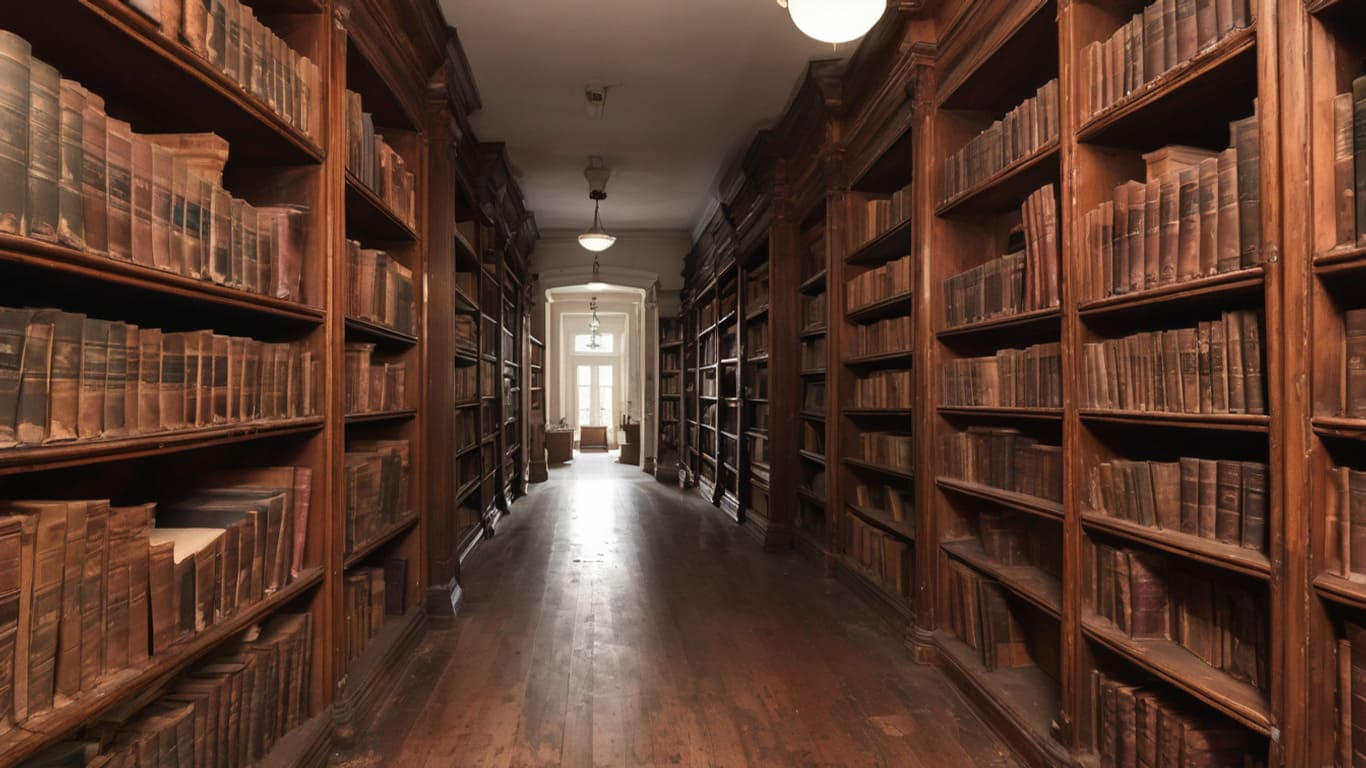
\includegraphics[height=52mm]{registry.jpg}
			
\includegraphics[height=52mm]{lazy.jpg}
		\end{figure}
	\end{frame}

	%Frame: client-server
	\begin{frame}
		\frametitle{Índices - Introdução e Motivação}
		\bigskip
		\begin{figure}[h]
			\centering
			
\includegraphics[height=52mm]{think-smartly.jpg}
		\end{figure}
	\end{frame}

	%Frame: client-server
	\begin{frame}
		\frametitle{Índices - Introdução e Motivação}
		\textbf{Vamos fazer o seguinte...}
		\bigskip
		\begin{itemize}
			\item Toda vez que um novo nascimento for registrado, anote o \texttt{nome completo} da pessoa em um pequeno cartão.
			\bigskip
			\item Neste cartão, escreva também o número do livro e a página onde foi o nascimento foi registrado
			\bigskip
			\item Guarde o cartão em um fichário alfabético
			\bigskip
			\item Da próxima vez que alguém solicitar uma certidão de nascimento de um sujeito chamado \textit{Fulano de Tal}: procure primeiramente pelo cartão e, em seguida, consulte o registro de nascimento no livro e página indicados.
		\end{itemize}
	\end{frame}

	%Frame: client-server
	\begin{frame}
		\frametitle{Conclusão}
		\textbf{Consequências da criação de índices:}
		\bigskip
		\begin{itemize}
			\item[\textbf{$\checkmark$}] Facilita enormemente o trabalho de pesquisa (este é o propósito de um índice)
			\bigskip
			\item[\textbf{$\times$}] Requer um espaço adicional de armazenamento (no nosso exemplo, além das estantes com os livros de registros, precisaríamos também de uma prateleira para armazenar os índices)
			\bigskip
			\item[$\times$] Dificulta o processo de adição de novos registros, pois sempre que um novo registro for criado, é necessário criar um cartão de índice a guardá-lo na ordem correta do fichário alfabético.
		\end{itemize}
	\end{frame}



	%Frame: client-server
	\begin{frame}
		\frametitle{Índices - Introdução e Motivação}
		Podemos indexar os registros de nascimento pelo \texttt{nome completo} da pessoa
		\bigskip
		
		Indexar = criar uma lista ordenada utilizando um dos campos de registro (nesse caso o \texttt{nome completo}) e indicando o local onde o registro completo pode ser encontrado (número do livro e a página)
		\bigskip
		
		Atenção: criar um índica não é significa criar uma cópia integral de todos os registros e organizá-los seguindo uma determinada ordenação.
		\bigskip
		
		Se assim fosse o cartório precisaria dobrar o tamanho da sala do arquivo para cada novo índice. 

	\end{frame}


\end{document}